\documentclass[aspectratio=169]{beamer}
\usetheme{Madrid}
\usecolortheme{beaver}
\usepackage[utf8]{inputenc}
\usepackage[T1]{fontenc}
\usepackage{tikz}
\usepackage{amssymb}
\usepackage{graphicx}
\setbeamertemplate{navigation symbols}{}
\setbeamercolor{title}{fg=white,bg=blue!55!black}
\setbeamercolor{frametitle}{fg=white,bg=blue!45!black}
\setbeamercolor{block title}{bg=blue!15,fg=black}
\setbeamercolor{block body}{bg=blue!5,fg=black}

\title{M9 — Interactive Apps}
\subtitle{A canvas app with real state: menu -> running -> results}
\author{ByteForge --- Grade 8 --- App Builder}
\date{}

\begin{document}

\begin{frame}
    \titlepage
\end{frame}

\begin{frame}{Today's Plan}
    \begin{itemize}
        \item Three Kinds of Bugs
        \item Trace Tables
        \item app\_state
        \item Guards \& Drawing
        \item A Growing List
        \item try/except
        \item[$\bigstar$] BOSS --- M9 Capstone
    \end{itemize}
\end{frame}

\begin{frame}{Three kinds of bugs, three different fixes}
    \Large
    A syntax error means Python can't parse your code. A logic error runs but gives the wrong answer. A runtime error crashes only on certain inputs. Naming which kind you have points to the right fix.
\end{frame}


\begin{frame}{app\_state — a real state machine}
    \Large
    \texttt{app\_state} is text ("menu", "running", "results") checked with if/elif — exactly Grade 7's state-machine idea, now controlling a real interactive app.

    \begin{center}
    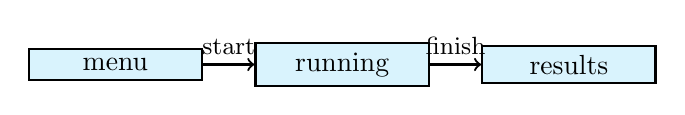
\begin{tikzpicture}[scale=0.9]

        \node[draw, thick, minimum width=2.2cm, fill=cyan!15] (m) at (0,0) {menu};
        \node[draw, thick, minimum width=2.2cm, fill=cyan!15] (r) at (3.2,0) {running};
        \node[draw, thick, minimum width=2.2cm, fill=cyan!15] (e) at (6.4,0) {results};
        \draw[->, thick] (m) -- (r) node[midway,above]{\small start};
        \draw[->, thick] (r) -- (e) node[midway,above]{\small finish};
    \end{tikzpicture}
    \end{center}
\end{frame}


\begin{frame}{Combining state, guards, and drawing}
    \Large
    Checking a divisor isn't 0 BEFORE dividing (a guard) prevents a real crash on a genuinely possible input — percentage, app\_state, and drawing, all connected.
\end{frame}


\begin{frame}{try/except — a different error, same pattern}
    \Large
    \texttt{int("abc")} raises a ValueError, caught with the exact same try/except pattern as any other error type — a real app can't just crash on unexpected input.
\end{frame}

\begin{frame}{Real-World Example}
    \Large
    Every real ATM walks through exactly this menu -> running -> results state pattern (select account -> processing -> show balance), with guard checks at every step (insufficient funds, wrong PIN) so it never just crashes on unexpected input.
\end{frame}


\begin{frame}{Image}
    \begin{center}
    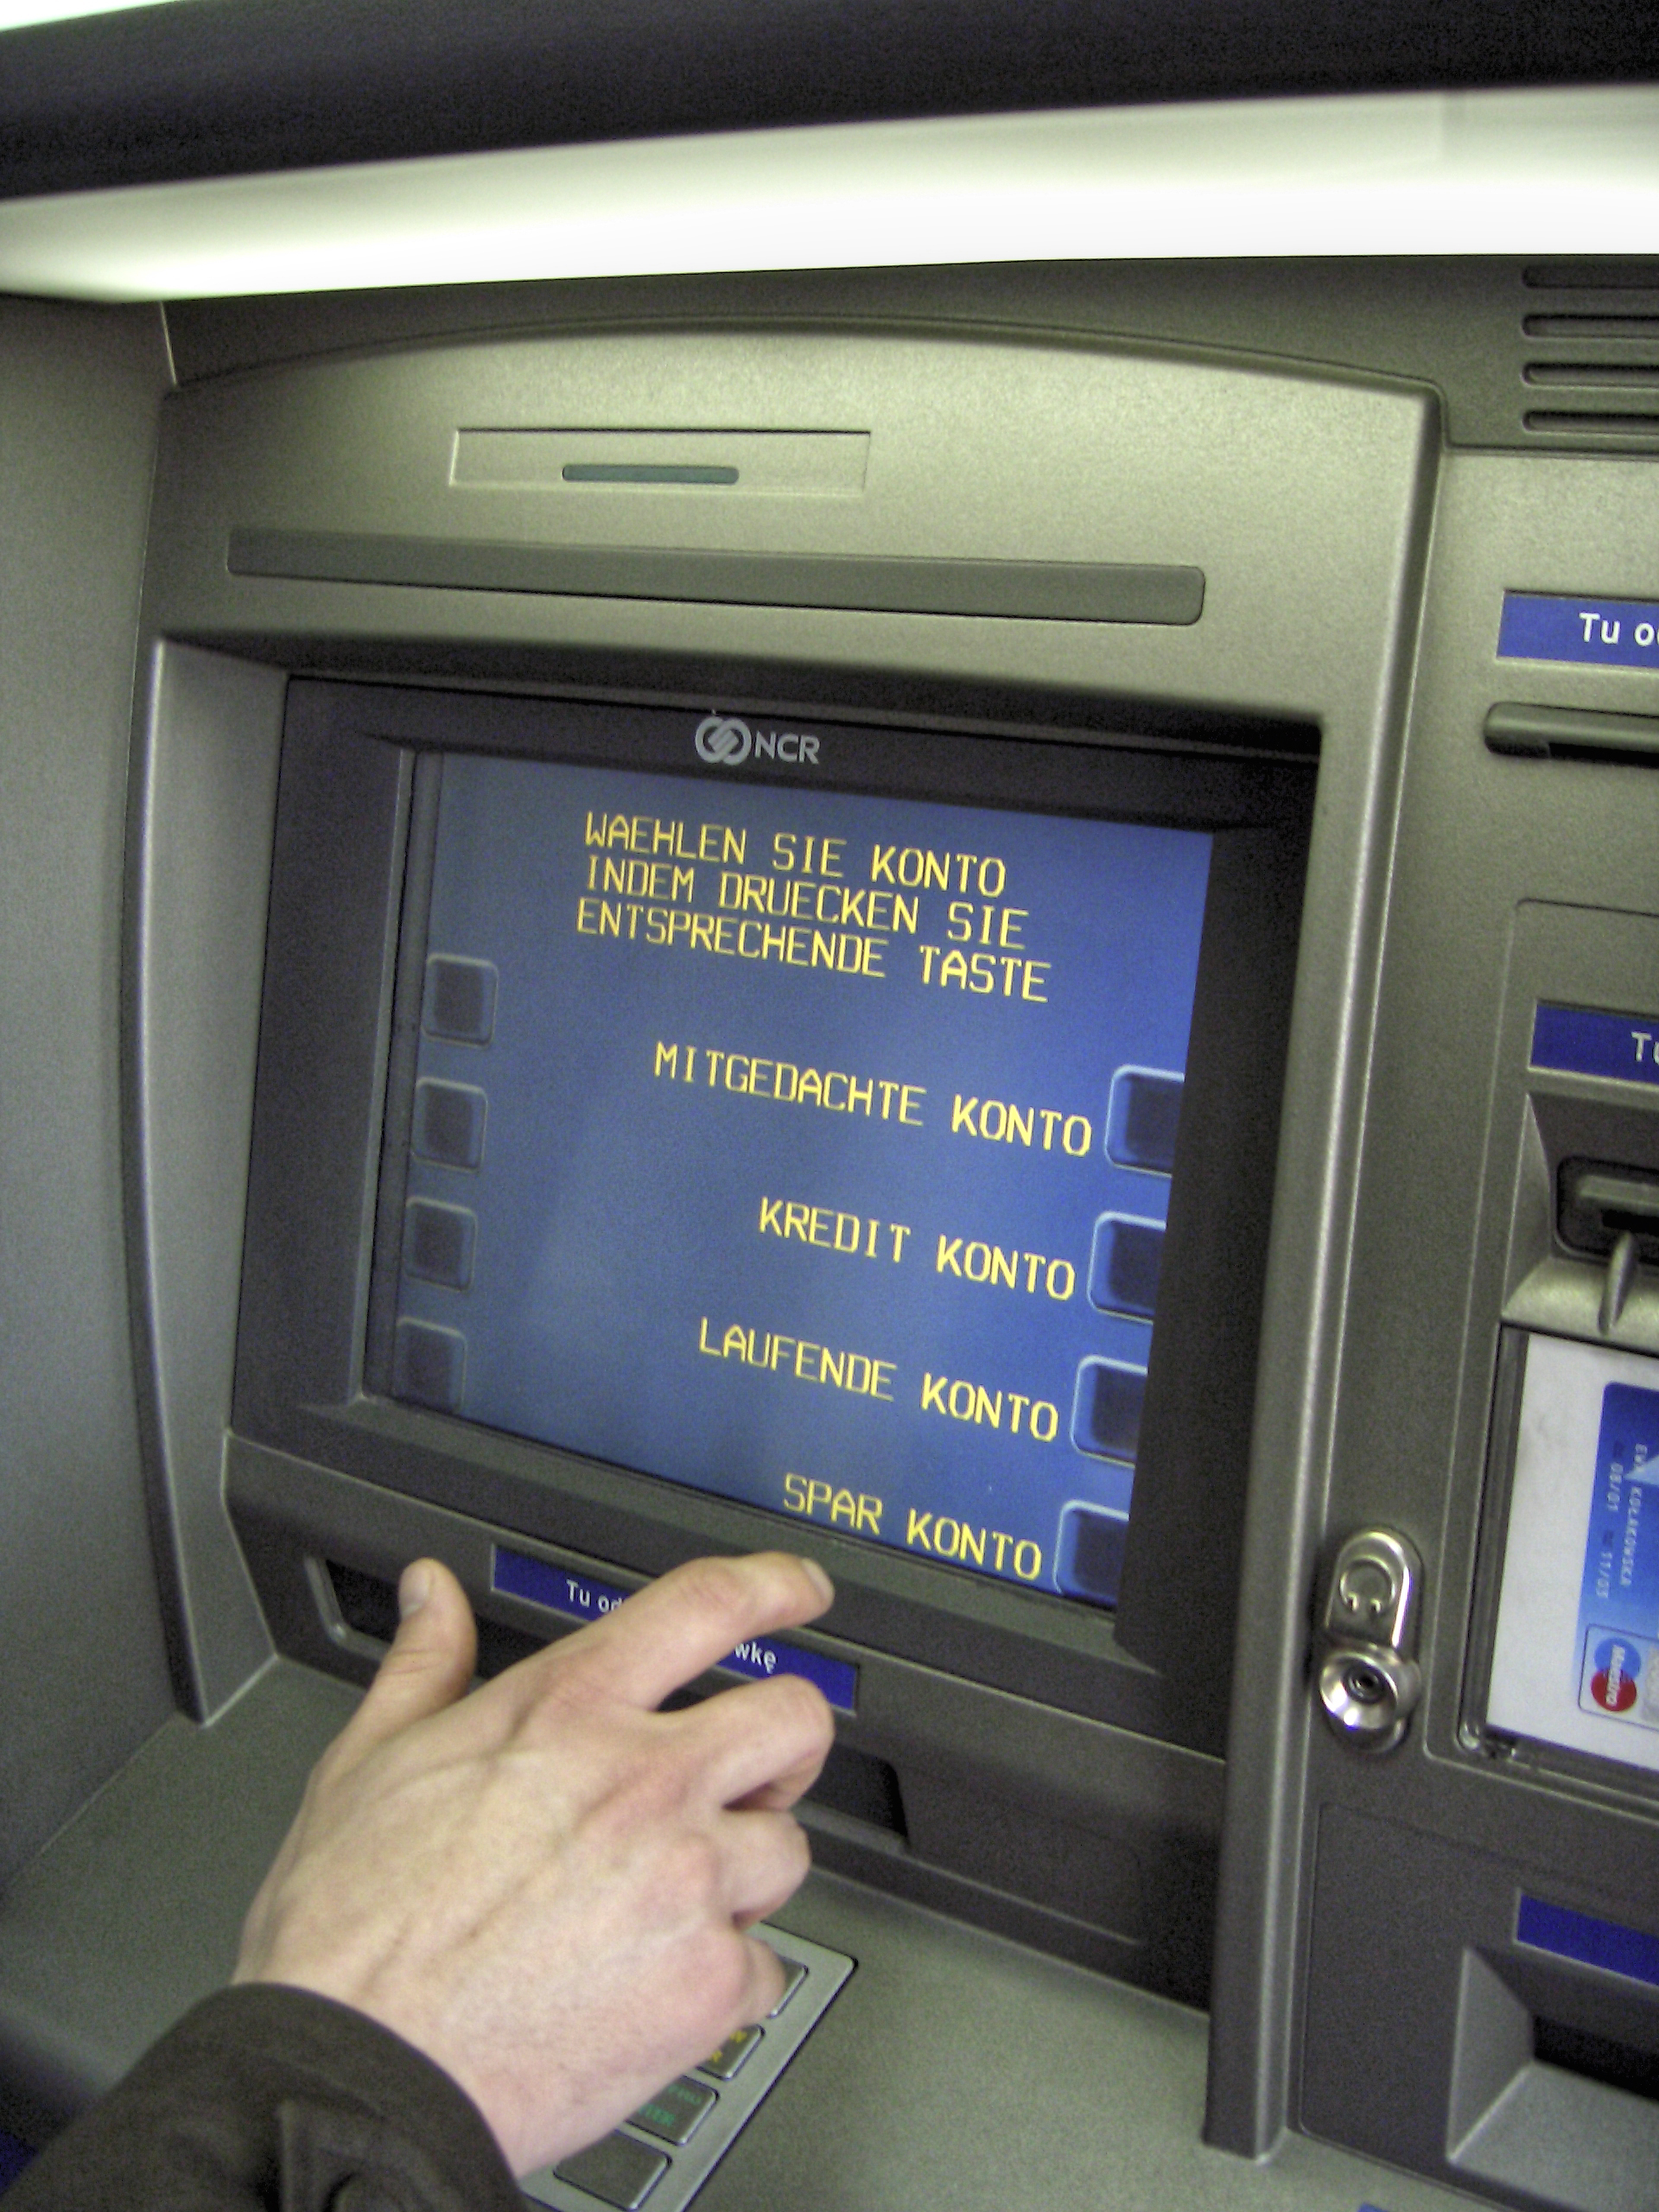
\includegraphics[width=0.5\textwidth]{images/atm.jpg}

    \large A real ATM walks through menu, then processing, then result --- the same state machine this chapter builds.

    \small ATM interface, Moritz Platt, public domain, via Wikimedia Commons
    \end{center}
\end{frame}

\begin{frame}{Let Them Discover}
    \Large
    Watch someone use an ATM (or recall using one). List the distinct "screens"/states it goes through from inserting a card to getting cash. Where do you think it needs a guard check (insufficient funds, wrong PIN)?
\end{frame}

\begin{frame}{Your Turn}
    \Large
    Open the student map, find \textbf{M9 — Interactive Apps}, and work through it
    hands-on --- everything you just saw, they now do themselves.
\end{frame}

\end{document}
